% $Id: notes.tex,v 1.6 2021/10/31 04:29:15 brandenb Exp $
%\documentclass{article}
\documentclass[twocolumn]{article}
\setlength{\textwidth}{160mm}
\setlength{\oddsidemargin}{-0mm}
\setlength{\textheight}{220mm}
\setlength{\topmargin}{-8mm}
\usepackage{graphicx,natbib}
\usepackage{bm,html,url}
\graphicspath{{./fig/}{./png/}}
\input macros
\title{Timing results for Lindgren and Triolith}
\author{Axel Brandenburg}
\date{March 12, 2014,~ $ $Revision: 1.6 $ $}
\begin{document}
\maketitle

\section{Code and test case}

For all tests, the {\sc Pencil Code} was used.
It is publicly available on \url{http://pencil-code.googlecode.com/},
where also detailed documentation is available.
The code uses explicit sixth order finite differences.
The time step is third-order.
In this sample, we run isothermal magnetohydrodynamics
in a periodic domain\footnote{Run directories are available on
\url{http://norlx51.nordita.org/~brandenb/pencil-code/timings/bforced/}}.
Power spectra are computed during the run, but our
current parallelization of the Fourier transform
requires that the meshpoint number is an integer multiple
of the product of processor numbers in the $y$ and $z$ directions
and the product of processor numbers in the $x$ and $y$ directions.
In addition, the number of processors in one direction should not
be so large that the number of mesh points per processor becomes
comparable to or less than the number of ghost zones (which is 6).

\section{Running the code}

To run the code, get one of the sample run directories, e.g.,
\url{http://norlx51.nordita.org/~brandenb/pencil-code/timings/bforced/512_4x16x32}.
The relevant file to be changed is \url{src/cparam.local}
\scriptsize
\begin{verbatim}
ncpus=2048,nprocx=4,nprocy=16,nprocz=ncpus/(nprocx*nprocy)
nxgrid=512,nygrid=nxgrid,nzgrid=nxgrid
\end{verbatim}
\normalsize
in particular the values of ncpus, nprocx, nprocy, and nxgrid.
Once they are chosen, say make, and submit
start\_run.csh.

\begin{figure}[b!]\begin{center}
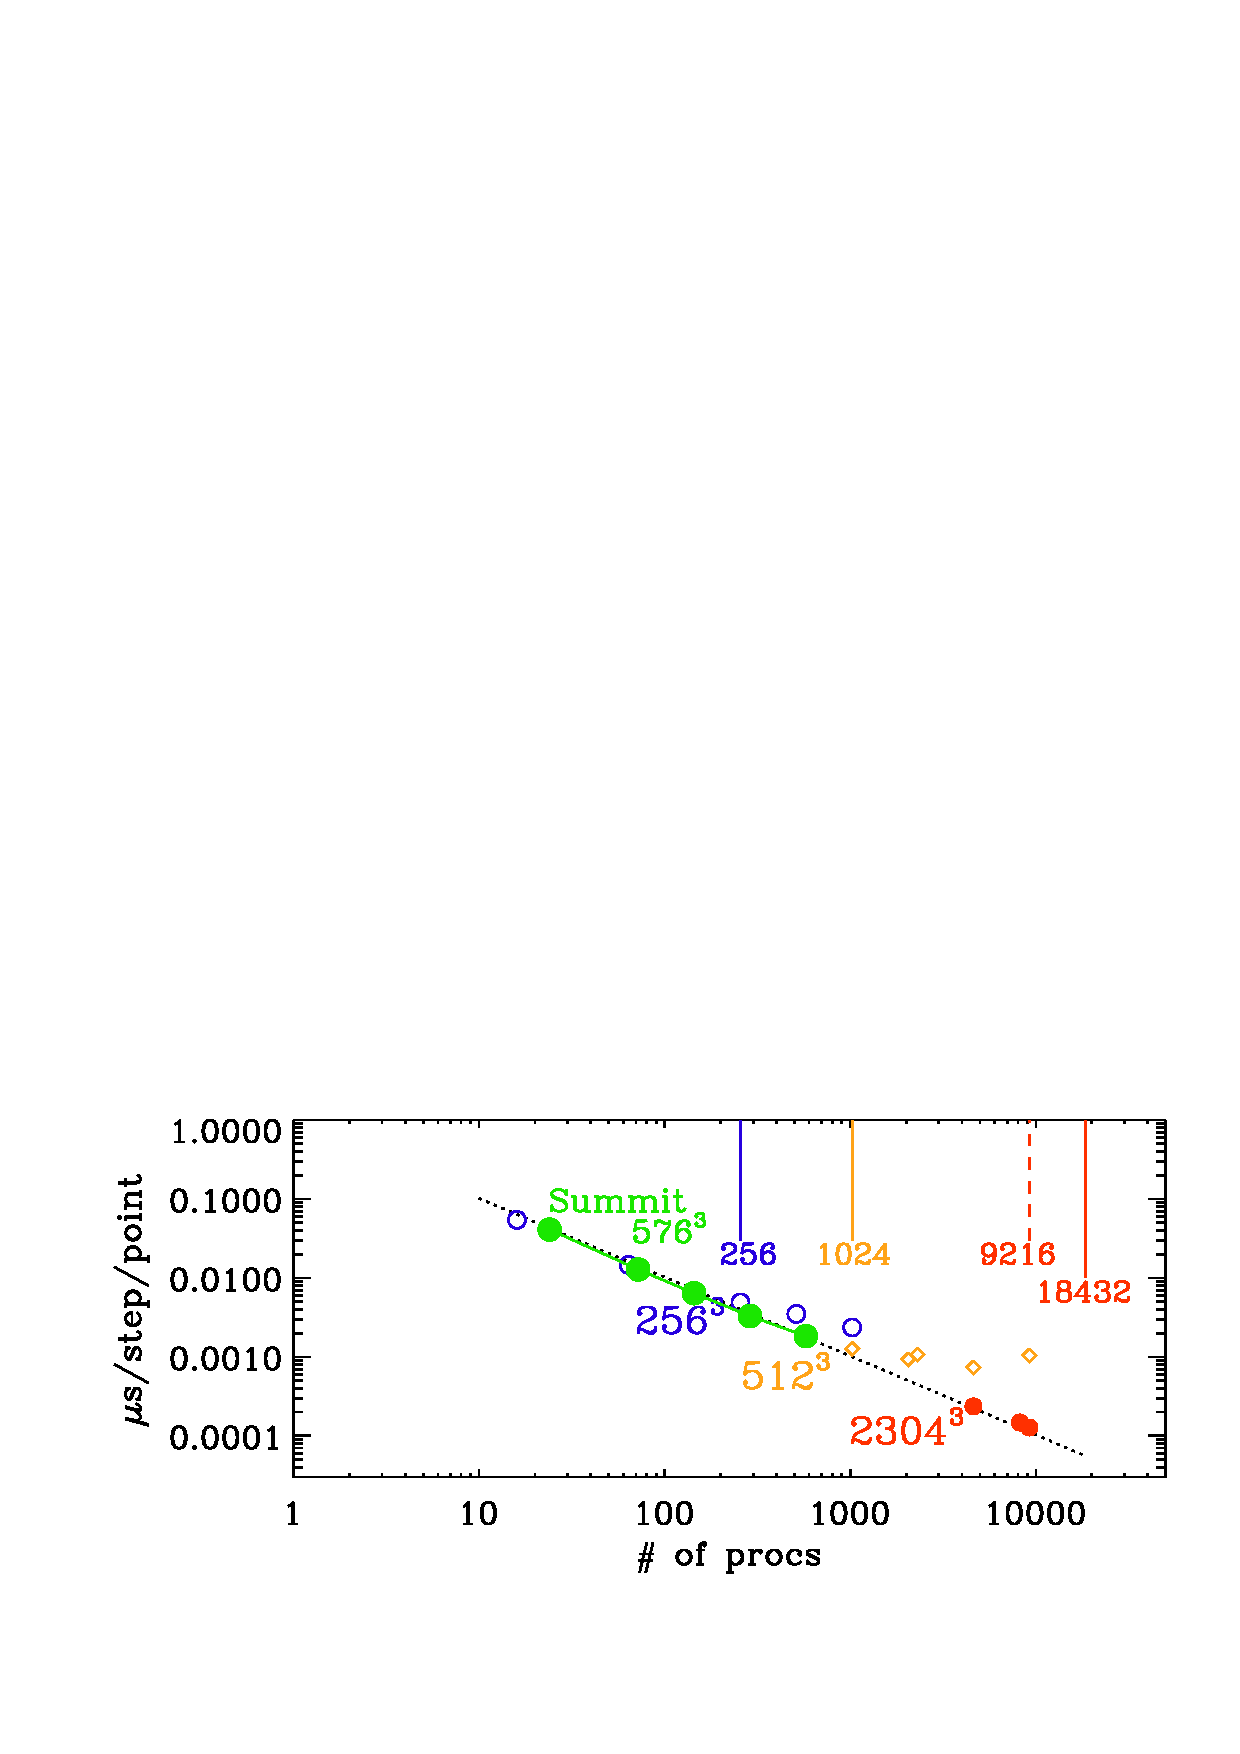
\includegraphics[width=\columnwidth]{ptriolith_strong}
\end{center}\caption[]{
Strong scaling on Triolith.
}\label{ptriolith_strong}\end{figure}

\section{Triolith}

On Triolith, strong scaling tests have been performed
for three mesh sizes.
The time per time step and mesh point is given for
different processor numbers and layouts.
Generally, it is advantageous to keep the number
of processors in the $x$ direction small.

\begin{table}[t!]\caption{
Triolith timings
}\vspace{12pt}\centerline{\begin{tabular}{rccc}
proc & $\displaystyle\frac{{\mu\rm s}}{\rm pt\;\;step}$ & resol. & layout \\
\hline
  16 &0.075& $128^3$ & 2x2x4  \\
  16 &0.065& $128^3$ & 1x4x4  \\
  16 &0.0544& $256^3$ & 1x4x4  \\  %256_1x4x4
  64 &0.0146& $256^3$ & 1x8x8  \\  %256_1x8x8
  64 &0.0164& $256^3$ & 2x4x8  \\
 256 &0.0049& $256^3$ & 1x16x16 \\ %256_1x16x16
 512 &0.0035& $256^3$ & 2x16x16 \\ %256_2x16x16
1024 &0.00236 &$256^3$ & 2x16x32 \\ %256_2x16x32
1024 &0.00127 &$512^3$ & 2x16x32 \\ %512_2x16x32
1024 &0.00129 &$512^3$ & 4x16x16 \\
2048 & $9.34{\times}10^{-4}$ &$ 512^3$&4x16x32 \\ %512_4x16x32
2304 & 0.00107 &$ 576^3$&4x18x32 \\  %576_4x18x32
4096 &$3.6{\times}10^{-4}$&$1024^3$&4x32x32 \\
4096 &$3.8{\times}10^{-4}$&$1024^3$&8x16x32 \\
4096 &$4.2{\times}10^{-4}$&$1024^3$&4x16x64 \\
4608 &$7.38{\times}10^{-4}$&$ 576^3$&8x18x32 \\ %576_8x18x32
4608 &$2.66{\times}10^{-4}$&$1152^3$&4x32x36 \\ %1152_4x32x36
4608 &$3.03{\times}10^{-4}$&$1152^3$&4x36x32 \\ %1152_4x36x32
4608 &$3.12{\times}10^{-4}$&$1152^3$&4x18x64 \\ %1152_4x18x64
4608 &$2.36{\times}10^{-4}$&$2304^3$&2x32x72 \\ %2304_2x32x72
8192 &$1.475{\times}10^{-4}$&$2048^3$&4x32x64 \\ %short2048pm1_kf60b
9216 & 0.00104 &$ 576^3$&16x18x32 \\ %576_16x18x32
9216 &$1.276{\times}10^{-4}$&$2304^3$&4x36x64 \\ %short2304pm1_kf60c
9216 &$1.30{\times}10^{-4}$&$2304^3$&4x32x72 \\ %2304_4x32x72
\label{Tsummary}\end{tabular}}\end{table}

{\em Comments}.~
Although on Triolith the number of processors per node is 16,
resolutions with one or two powers of 3 (such as 576) still work well.
Furthermore, the number of processors above which the scaling becomes
poor increases quadratically with the number of mesh points.
This implies that the RAM per processor increases linearly with
the problem size per direction.
However, this will not be a limitation, because even for $2304^3$
meshes, the required RAM is still below 100 MB.
%    256     512    1152    2304
%    256    1152    4608   18432
%    7.3    13.0    37.2   74.32

\section{Lindgren}

On Lindgren, we have performed weak scaling tests and compare
with weak scaling results for Triolith.
Triolith is about twice as fast as Lindgren.

\begin{table}[h]\caption{
Lindgren timings
}\vspace{12pt}\centerline{\begin{tabular}{rccc}
proc & $\displaystyle\frac{{\mu\rm s}}{\rm pt\;\;step}$ & resol. & layout \\
\hline
1536&0.00171&$512^2{\times}384$& 2x32x24 \\
2048&0.00129&$512^2{\times}1024$&1x32x64 \\
2048&0.00129&$1024^2{\times}2048$&1x32x64 \\
4096&$4.6{\times}10^{-4}$&$2048^3$&4x16x64 \\
9216&$2.36{\times}10^{-4}$&$2304^3$&4x48x48 \\
\label{Tsummary}\end{tabular}}\end{table}

\begin{figure}[h!]\begin{center}
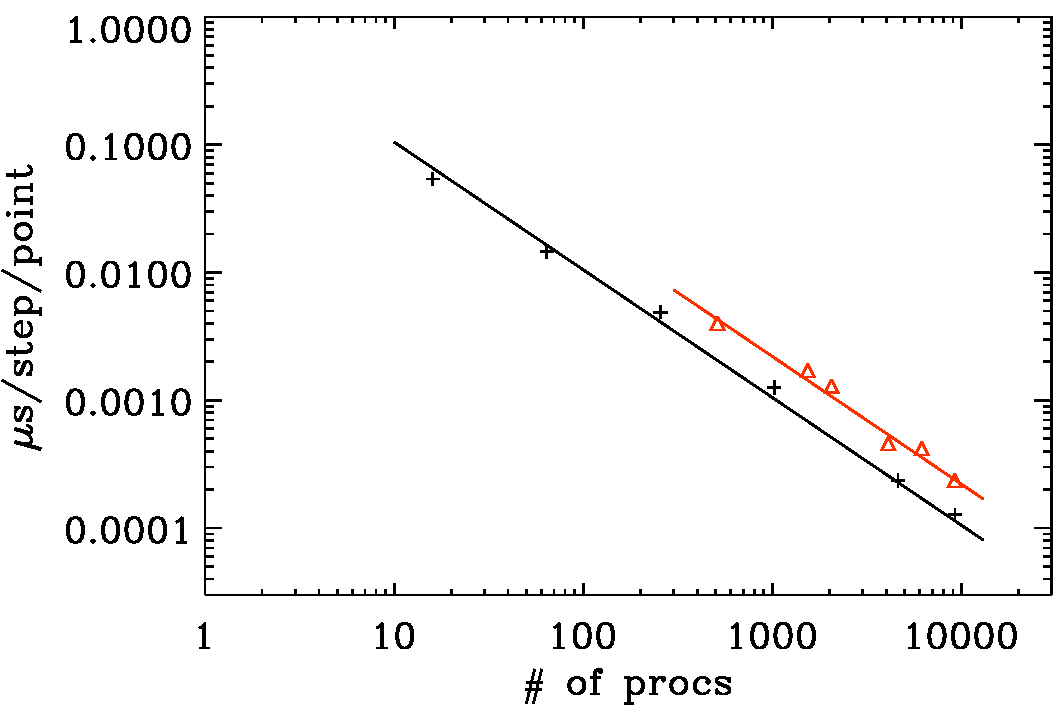
\includegraphics[width=\columnwidth]{pcomp_performance_2014}
\end{center}\caption[]{
Comparison Triolith (black, plus signs)
and Lindgren (red, triangles).
Weak scaling.
}\label{pcomp_performance_2014}\end{figure}

%\section{Archer}

%Compilation with
%\begin{verbatim}
%ftn  -O3 -ffree -e m -J experimental -J 
%\end{verbatim}

%\begin{itemize}
%\item
%\end{itemize}

%r e f
%\begin{thebibliography}{}

%\bibitem[Biskamp \& M\"uller(1999)]{BM99}
%Biskamp, D., \& M\"uller, W.-C.\yprl{1999}{83}{2195}

%\end{thebibliography}

\vfill\bigskip\noindent\tiny\begin{verbatim}
$Header: /var/cvs/brandenb/tex/pencil-code/performance/notes.tex,v 1.6 2021/10/31 04:29:15 brandenb Exp $
\end{verbatim}

\end{document}
